\documentclass[11pt,letterpaper]{article}
\usepackage[left=2.5cm,right=3cm]{geometry}
\usepackage[T1]{fontenc}
%\usepackage{newtxtext,newtxmath}
\usepackage{graphicx}
\usepackage{enumitem}
\setlength{\parindent}{0pt}
\setlength{\parskip}{2.5pt}
\newcommand{\heading}[1]{\par\vspace{3pt}{\Large\bfseries #1}\par\vspace{0pt}}





\begin{document}


\begin{center}
{\LARGE\bfseries The sound of silencing}\par
\vspace{2pt}
{\normalsize\bfseries Gene regulation through microRNA in the human and chimpanzee brain}\par
\vspace{2pt}
{\normalsize\bfseries Author: Bjoern Muetzel}\par
\vspace{2pt}
{\small Executive summary \enspace\textbullet\enspace November 2026}
\end{center}
\vspace{-4pt}

\heading{Summary}
MicroRNAs (miRNAs) are small RNA molecules that silence or reduce the production of proteins from messenger RNAs (mRNAs). There are about 2000 miRNAs in our genome that modulate the expression of about 60\% of all genes, where each miRNA regulates about 100 - 400 genes through binding with its seed sequence (see Figure 1). We examined whether miRNA regulation shows different patterns in humans and chimpanzee brains. The central question is whether the \emph{network} of miRNA-gene interactions changes differently with age in humans and chimpanzees. A related second goal was to identify functional groups of genes that are expressed differently between humans and chimpanzees during early development (<100 days).\\

\heading{Data}
We used published measurements from \cite{so} from the \textbf{prefrontal cortex}, a brain region important for planning and complex thinking, in humans, chimpanzees, and rhesus macaques. The cleaned data contained \textbf{11,667 genes across 58 mRNA profiles} and \textbf{198 detected miRNAs across 27 miRNA profiles}. As the experiments covered only partly overlapping samples, the network analysis paired profiles by species and age; these are not necessarily two measurements from the same individual. We compared \textbf{17 human-chimpanzee matched profiles} (7 human, 10 chimpanzee), using approximate adjustments for species' different developmental timelines. The macaque data was used in the regression analysis and the network analysis, but not in the humans-chimpanzee comparison during early development.\\

\heading{Questions}
We studied four complementary questions:
\begin{itemize}[leftmargin=1.35em,topsep=1pt,itemsep=1pt,parsep=0pt]
\item \textbf{Regression analysis:} How much does gene and miRNA expression vary with species and age?
\item \textbf{Autism:} Are genes differing in expression between infant humans and chimpanzees (< 100 days old) unusually likely to be autism-associated?
\item \textbf{Gene Ontology:} Which broad biological functions distinguish the species' expression patterns in this fourth trimester?
\item \textbf{Network analysis:} Do patterns of miRNA-gene regulation shift differently during life between humans and chimpanzees?\\
\end{itemize}

\newpage

\heading{Results}

The precursory regression analysis shows that age and species together accounted for about \textbf{38\%} of observed mRNA variation and \textbf{50\%} of miRNA variation on average in the fitted models. The main results are:\\


{\large \textbf{Human-chimpanzee differences during early development}}

\textbf{Gene expression differences.}
We analyzed gene expression differences using the pylimma package \cite{ri}. In nine infant (<100 days old) human/chimpanzee profiles, we identified \textbf{140 candidate genes} with differences in expression (62 higher in humans, 78 in chimpanzees; false-discovery-rate threshold $<0.15$). 

\textbf{Autism and biological functions.} Those 140 genes showed \textbf{no statistically significant enrichment} for SFARI autism-associated genes (one-sided Fisher tests). We then examined significant cagegories using the tool GofuncR (\cite{gr},\cite{pr}). A broader ranking of gene expression found \textbf{10 human-higher} refined Gene Ontology categories, notably transcription and RNA processing, and \textbf{30 chimpanzee-higher} categories, notably synaptic activity, ion transport and cellular energy processes (family-wise error rate $\leq0.05$).\\


{\large \textbf{miRNA-mRNA network life-history analyis}}

MiRNAs with the same short \emph{seed sequence} can be grouped into a family. The miRDB database links these families to possible target genes (see Figure 1).

\begin{center}
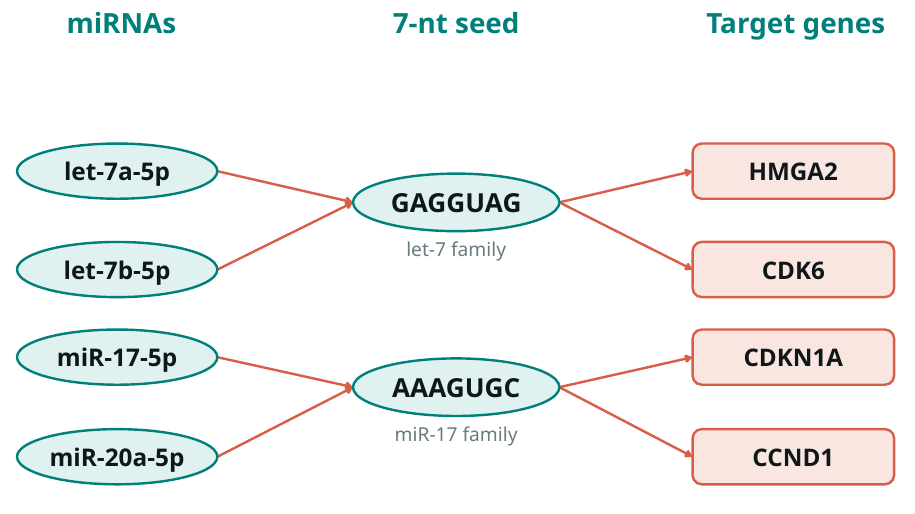
\includegraphics[width=0.92\linewidth,height=2.35in,keepaspectratio]{mirna_seed_targets.png}\\[-1pt]
{\small\textbf{Figure 1} Several microRNAs can share a common seed sequence and  regulate the same target genes.}
\end{center}


For each of the 17 (7 humans, 10 chimpanzees) age-matched profiles, we combined measured miRNA and mRNA expression with the predicted links. The nodes of our network are the seeds on one side that regulate the gene/ mRNA nodes on the other side. A link or edge received a higher score when the miRNA family belonging to a seed was relatively highly expressed and its target gene relatively low, giving us an \textbf{computational indicator of regulation}. Six network statistics were analysed. Among these two showed significant differences (see Figure 2):\\

\textbf{Target in-strength variation (CV).} This network parameter measures how unequal the target genes are activated. For each gene, we averaged the scores of the predicted edges pointing to it. We then asked how much these averages differed \emph{from one target gene to another}. A high value means some genes have considerably higher average regulation scores than others. \textbf{This unevenness declined more with age in humans than in chimpanzees} (FDR $=0.0132$). Put simply, the estimated regulatory activity became \emph{more evenly distributed across target genes} in the human samples.\\

\textbf{Edge-score dispersion.} This parameter measures how equal or unequal the individual connections are.  Here we looked at all individual predicted miRNA-gene connections, rather than first averaging by target gene. This measures how different the link scores are from one another. \textbf{Their spread also declined more with age in humans} (FDR $=0.0462$). In everyday terms, the network's links became \emph{more similar in their estimated activity} during human development.\\

These findings are related but distinct: the first concerns \textbf{differences between genes}; the second concerns \textbf{differences between individual predicted links}. Both were significant after correcting for testing six network parameters, using 5,000 permutation tests.

\begin{center}
\begin{minipage}[t]{0.487\linewidth}
\centering
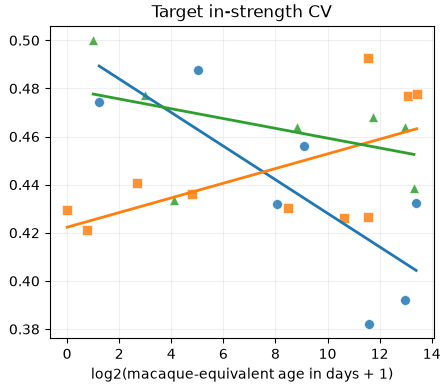
\includegraphics[width=\linewidth,height=2.53in,keepaspectratio]{target_instrength_cv.png}\\[-2pt]
{\footnotesize\bfseries Target in-strength variation}\\[-1pt]
{\footnotesize Human-chimp slope difference $-0.00999$}
\end{minipage}\hfill
\begin{minipage}[t]{0.487\linewidth}
\centering
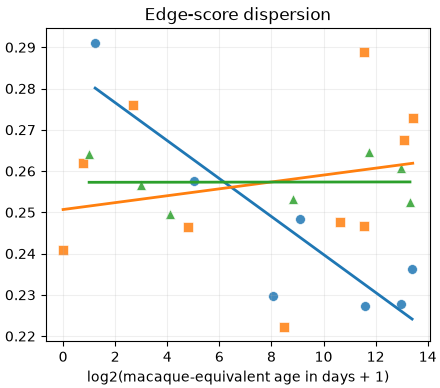
\includegraphics[width=\linewidth,height=2.53in,keepaspectratio]{edge_score_dispersion.png}\\[-2pt]
{\footnotesize\bfseries Edge-score dispersion}\\[-1pt]
{\footnotesize Human-chimp slope difference $-0.00544$}
\end{minipage}
\\[2pt]
{\small\textbf{Figure 2.} Network measures versus developmentally aligned age. Blue circles: humans; orange squares: chimpanzees; green triangles: macaques. Lines are descriptive fits.}
\end{center}

\newpage

\heading{Discussion}
The results suggest that, over development, the \textbf{pattern of predicted miRNA-gene activity becomes more even in humans relative to chimpanzees}. This does \emph{not} mean that miRNAs necessarily silence more genes or fewer genes, nor does it establish that the difference caused human-specific brain evolution. It is, however, an interesting and promising \textbf{network-level signal} that merits further investigation.



\begin{thebibliography}{Pr}
\bibitem[So]{so}
Somel, M., Liu, X., Tang, L. et al. \textit{MicroRNA-driven developmental remodeling in the brain distinguishes humans from other primates.} PLoS Biology, 9(12), (2011).

\bibitem[Ri]{ri}
Ritchie, M. E., Phipson, B., Wu, D. et al. \textit{limma powers differential expression analyses for RNA-sequencing and microarray studies.}, Nucleic Acids Research, 43(7), e47 (2015).

\bibitem[Gr]{gr}
Grote, S. \textit{GOfuncR: Gene Ontology enrichment using FUNC.}, Bioconductor R package. DOI: 10.18129/B9.bioc.GOfuncR

\bibitem[Pr]{pr}
Prüfer, K., Muetzel, B., Do, H.-H., et al. \textit{FUNC: a package for detecting significant associations between gene sets and ontological annotations.} BMC Bioinformatics, 8, 41, (2007)

\end{thebibliography}

\end{document}
